% CS224W Project Milestone (Project Type 1: Real-world application)
% Overleaf: put neurips_2022.sty next to this file, plus the folders `explore/` and `tables/`
% from milestone_results.zip (produced by the Colab notebook). Until they are there, the
% report still compiles, with clearly marked placeholders.
\IfFileExists{neurips_2022.sty}{%
  \documentclass{article}
  \usepackage[final,nonatbib]{neurips_2022}
}{%
  \documentclass[10pt]{article}
  \usepackage[textwidth=5.5in,textheight=9in,centering]{geometry}
  \usepackage{times}
}

\usepackage[utf8]{inputenc}
\usepackage[T1]{fontenc}
\usepackage[colorlinks=true,linkcolor=blue!60!black,citecolor=blue!60!black,urlcolor=blue!60!black]{hyperref}
\usepackage{url}
\usepackage{booktabs}
\usepackage{amsmath,amsfonts}
\usepackage{microtype}
\usepackage{xcolor}
\usepackage{graphicx}
\usepackage{tikz}
\usetikzlibrary{positioning,arrows.meta}

% Red markers for the few sentences to finish once results are in.
\newcommand{\todo}[1]{\textcolor{red!70!black}{[TODO: #1]}}

% Dataset statistics: defaults, overwritten by explore/stats.tex from the notebook.
\def\NumTables{15}\def\NumRows{5.4M}\def\NumCols{140}
\def\RowsOutcomeTrain{--}\def\RowsOutcomeVal{--}\def\RowsOutcomeTest{--}
\def\PosOutcomeTrain{--}\def\PosOutcomeVal{--}\def\PosOutcomeTest{--}
\def\RowsAdverseTrain{--}\def\RowsAdverseVal{--}\def\RowsAdverseTest{--}
\def\MedianAdverseTrain{--}\def\MedianAdverseVal{--}\def\MedianAdverseTest{--}
\def\PtfAdverseTrain{--}\def\PtfAdverseVal{--}\def\PtfAdverseTest{--}
\IfFileExists{explore/stats.tex}{\input{explore/stats.tex}}{}

\IfFileExists{tables/main_rows.tex}{\def\ResultRows{\csname @@input\endcsname tables/main_rows.tex }}% primitive input: works inside tabular
  {\def\ResultRows{\multicolumn{6}{c}{\todo{run the notebook and upload \texttt{tables/main\_rows.tex}}} \\}}

\newcommand{\fig}[2]{\IfFileExists{#1}{\includegraphics[width=#2]{#1}}%
  {\fbox{\parbox[c][1.1in][c]{#2}{\centering\small\todo{run the notebook}\\\texttt{\detokenize{#1}}}}}}

\title{When Does Relational Structure Pay Off?\\
Accuracy--Cost Tradeoffs of Relational Graph Models\\for Clinical Trial Outcome Prediction\\
\large Project Milestone}

\author{%
  Manel Bermad\\
  Stanford University\\
  \texttt{mbermad@stanford.edu}
}

\date{}
\begin{document}
\maketitle

\vspace{-1.2em}
\noindent\textbf{Project type:} 1 (Real-world application of GNNs).
\textbf{Code:} \url{https://github.com/mbermad/relational-trials}
(Colab: \texttt{notebooks/milestone\_colab.ipynb}).

\section{Problem and progress}

Most clinical trials fail, and the information that predicts failure is \emph{relational}: a
trial shares sponsors, conditions, interventions and sites with thousands of trials whose
outcomes are known. We ask when learning directly on that structure, with graph neural
networks over the database, beats strong tabular baselines, at what cost, and what the models
learn. The motivation is concrete: on RelBench's published single-run results for our main
task, a LightGBM baseline (AUROC 0.689) is ahead of the reference GNN (0.669), and the two tie
on adverse-event regression (NMAE 0.129 each)~\cite{relbench_leaderboard}.

\textbf{Done for the milestone:} (1) a reproducible pipeline that loads the data through
RelBench~3 and evaluates on held-out test labels offline; (2) a shared evaluation harness
(metrics, 3 seeds, 95\% confidence intervals, paired bootstrap, run logging); (3) two LightGBM
baselines, one with leakage-safe relational aggregates; (4) the RDL baseline, a heterogeneous
GraphSAGE with temporal sampling; (5) unit and end-to-end tests, including tests that features
never see the future. Table~\ref{tab:results} reports all models on both tasks.

\section{Dataset and processing}

\paragraph{Data.} We use \texttt{rel-trial} from RelBench~\cite{robinson2024relbench}, a
relational database built from ClinicalTrials.gov via the AACT database~\cite{aact}:
\NumTables{} tables, about \NumRows{} rows and \NumCols{} columns, covering trials that started
from 2000 onward (Figure~\ref{fig:schema}). Tables available when a trial starts (design,
eligibility, sponsor and site links) are timestamped at its start date; tables only known when
it ends (outcomes, analyses, adverse events, withdrawals) are timestamped at its completion
date. The time-based splits put validation seeds at 2020-01-01 and test seeds from 2021-01-01.

\begin{figure}[t]
\centering
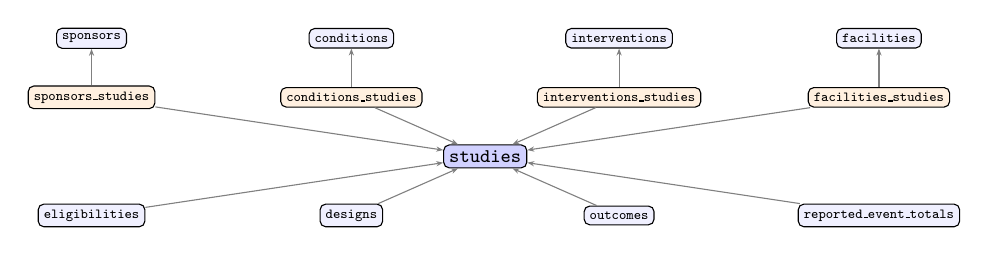
\begin{tikzpicture}[
  tbl/.style={draw, rounded corners=2pt, font=\tiny\ttfamily, inner sep=2pt, fill=blue!6},
  jn/.style={draw, rounded corners=2pt, font=\tiny\ttfamily, inner sep=2pt, fill=orange!12},
  lk/.style={draw, gray, -{Stealth[length=2.5pt]}}]
  \node[tbl, fill=blue!18, font=\scriptsize\ttfamily\bfseries] (st) at (0,0) {studies};
  \foreach \x/\a/\b in {-5/sp/sponsors, -1.7/co/conditions, 1.7/iv/interventions, 5/fa/facilities} {
    \node[tbl] (\a) at (\x,1.5) {\b};
    \node[jn] (j\a) at (\x,0.75) {\b\_studies};
    \draw[lk] (j\a) -- (\a); \draw[lk] (j\a) -- (st);
  }
  \foreach \x/\a/\b in {-5/el/eligibilities, -1.7/de/designs, 1.7/ou/outcomes, 5/ae/reported\_event\_totals} {
    \node[tbl] (\a) at (\x,-0.75) {\b};
    \draw[lk] (\a) -- (st);
  }
\end{tikzpicture}
\caption{\texttt{rel-trial} schema (13 of 15 tables; \texttt{outcome\_analyses} and
\texttt{drop\_withdrawals} also link to \texttt{studies}). Arrows are primary--foreign key
links, which become edges in the relational entity graph; orange tables are junction tables.}
\label{fig:schema}
\vspace{-0.8em}
\end{figure}

\paragraph{Tasks.} \texttt{study-outcome}: for trials completing in the year after a seed
time, predict whether the trial meets its primary outcome (binary; AUROC). \texttt{study-adverse}:
predict the number of patients with serious adverse events or death (regression). RelBench~3
scores regression with NMAE, the MAE divided by the training-target standard deviation; we
report NMAE and raw MAE. Table~\ref{tab:splits} gives split sizes.

\begin{table}[h]
\centering\small
\caption{Label tables. Adverse-event counts are heavy-tailed (Figure~\ref{fig:data}, right).}
\label{tab:splits}
\begin{tabular}{lccc}
\toprule
 & Train & Val & Test \\
\midrule
\texttt{study-outcome}: rows (share positive) & \RowsOutcomeTrain{} (\PosOutcomeTrain) & \RowsOutcomeVal{} (\PosOutcomeVal) & \RowsOutcomeTest{} (\PosOutcomeTest) \\
\texttt{study-adverse}: rows (median, 95th pct.) & \RowsAdverseTrain{} (\MedianAdverseTrain, \PtfAdverseTrain) & \RowsAdverseVal{} (\MedianAdverseVal, \PtfAdverseVal) & \RowsAdverseTest{} (\MedianAdverseTest, \PtfAdverseTest) \\
\bottomrule
\end{tabular}
\end{table}

\begin{figure}[t]
\centering
\fig{explore/trials_per_year.png}{0.48\linewidth}\hfill
\fig{explore/adverse_distribution.png}{0.48\linewidth}
\caption{Left: trials by start year, with the validation and test boundaries. Right: the
adverse-event target on a log scale.}
\label{fig:data}
\vspace{-0.8em}
\end{figure}

\paragraph{Processing and leakage control.} RelBench~3 loads the database from the Hugging
Face Hub; we read test labels with \texttt{mask\_input\_cols=False}, as RelBench's own
evaluator does, so every run is scored offline. Two rules keep every model honest. (1) A
prediction at seed time $t$ only uses database rows dated $\le t$; for the GNN this is
RelBench's temporal neighbor sampler, and for LightGBM our feature code applies the same
filter. (2) Another trial's label is only used once it is known: its label time plus the
task's one-year window must be $\le t$. Tests on hand-built examples check both rules.

\section{Models}

\paragraph{LightGBM on the trial's own table}~\cite{ke2017lightgbm}. Categorical and numeric
columns of \texttt{studies}, date features, and a 32-dimensional TF-IDF/SVD summary of the
trial's titles. This asks how far a model gets without any other table.

\paragraph{LightGBM with relational aggregates.} Adds hand-engineered joins in the style of
Deep Feature Synthesis~\cite{kanter2015dfs}: columns of the one-to-one \texttt{designs} and
\texttt{eligibilities} tables; counts of rows in every table linked to the trial; and, for each
linked sponsor, condition, facility and intervention, how many trials it started before $t$
and the smoothed mean label of its past trials known by $t$, averaged and maxed over the
trial's links. This is the strongest non-graph baseline we can build from the same
information the GNN sees.

\paragraph{RDL baseline.} Following Relational Deep Learning~\cite{fey2024rdl}, each row is a
node typed by its table and each primary--foreign key link a typed edge. PyTorch
Frame~\cite{hu2024frame} encodes each node's columns (text with 300-d GloVe~\cite{pennington2014glove})
into $h_v^{(0)}$, to which we add an encoding of the node's age relative to the seed time.
Two layers of heterogeneous GraphSAGE~\cite{hamilton2017sage} in PyG~\cite{fey2019pyg} update
\begin{equation*}
h_v^{(\ell+1)} = \mathrm{ReLU}\Big(\mathrm{LayerNorm}\Big(\sum_{r \in \mathcal{R}(v)}
\Big[W_{r,\text{self}}^{(\ell)} h_v^{(\ell)} + W_r^{(\ell)}
\sum_{u \in \mathcal{N}_r(v),\, t_u \le t} h_u^{(\ell)}\Big]\Big)\Big),
\end{equation*}
where $\mathcal{R}(v)$ are the edge types into $v$'s table and $t$ is the seed time; an MLP
reads out the trial node. We use RelBench's reference settings: 128 channels,
128 and 64 sampled neighbors per hop, Adam with learning rate 0.005, 10 epochs, binary
cross-entropy or L1 loss, and model selection on validation.

\section{Evaluation protocol}

Every model uses the same splits and seeds (0, 1, 2) and logs one record per run with
validation and test metrics, training time, inference latency and peak GPU memory. LightGBM
variants get the same tuning budget (20 random-search trials on validation), then retrain per
seed; the GNN uses fixed reference hyperparameters. We report the mean and a $t$-based 95\%
confidence interval over seeds; for model comparisons in the final report we add a paired
bootstrap over test trials.

\section{Preliminary results}

\begin{table}[t]
\centering\small
\caption{Mean over 3 seeds, $\pm$ 95\% CI. AUROC: higher is better; NMAE and MAE: lower is
better. Bold marks the best in each column. Bottom rows: RelBench's published single runs.}
\label{tab:results}
\setlength{\tabcolsep}{4pt}
\begin{tabular}{lccccc}
\toprule
 & \multicolumn{2}{c}{Outcome AUROC $\uparrow$} & \multicolumn{3}{c}{Adverse events $\downarrow$} \\
\cmidrule(lr){2-3}\cmidrule(lr){4-6}
Model & Val & Test & NMAE val & NMAE test & MAE test \\
\midrule
\ResultRows
\bottomrule
\end{tabular}
\vspace{-0.5em}
\end{table}

\todo{Two or three sentences once the table is filled. Answer: (1) Do our LightGBM and RDL
numbers land near RelBench's (0.689 / 0.669 AUROC, 0.129 NMAE)? Explain any gap. (2) Do
relational aggregates improve LightGBM, and by how much relative to the CI? (3) How does the
GNN compare with the aggregate baseline? (4) One line on training time, from
\texttt{tables/runtime\_rows.tex}.}

\section{Next steps}

\begin{enumerate}
\item \textbf{By Nov 24:} RelGNN~\cite{chen2025relgnn} and RelGT~\cite{dwivedi2026relgt} from
their official code, behind the same harness and seeds.
\item \textbf{C1, tradeoffs (by Dec 1):} accuracy against training time, inference latency and
memory; slices by phase and condition; calibration; robustness when training stops at earlier
years; randomly rewired foreign keys as a control.
\item \textbf{C2, explanations:} attributions per table and relation type, validated with a
deletion test.
\item \textbf{C3, hybrid:} GNN trial embeddings (already exported by our pipeline) as features
for LightGBM, compared on accuracy and serving cost.
\end{enumerate}

\paragraph{Questions for our mentor.} (1) Is retraining with earlier cutoff years a sound way
to measure robustness over time on \texttt{rel-trial}, or would you suggest another protocol?
(2) Should C2's deletion test retrain the model or only mask relations at inference?
(3) Would a careful version of this comparison be a reasonable workshop submission?

\small
\begin{thebibliography}{99}

\bibitem{robinson2024relbench} J.~Robinson, R.~Ranjan, W.~Hu, K.~Huang, J.~Han, A.~Dobles, M.~Fey, J.~E.~Lenssen, Y.~Yuan, Z.~Zhang, X.~He, and J.~Leskovec. RelBench: A benchmark for deep learning on relational databases. In \emph{NeurIPS Datasets and Benchmarks Track}, 2024. \href{https://arxiv.org/abs/2407.20060}{arXiv:2407.20060}.

\bibitem{relbench_leaderboard} RelBench leaderboard entries ``LightGBM'' and ``GNN'' (RelBench baselines), \url{https://github.com/stanford-star/relbench/tree/main/leaderboard}, accessed November 2026.

\bibitem{fey2024rdl} M.~Fey, W.~Hu, K.~Huang, J.~E.~Lenssen, R.~Ranjan, J.~Robinson, R.~Ying, J.~You, and J.~Leskovec. Position: Relational deep learning -- graph representation learning on relational databases. In \emph{ICML}, PMLR 235, 2024. \href{https://proceedings.mlr.press/v235/fey24a.html}{proceedings.mlr.press/v235/fey24a}.

\bibitem{ke2017lightgbm} G.~Ke, Q.~Meng, T.~Finley, T.~Wang, W.~Chen, W.~Ma, Q.~Ye, and T.-Y.~Liu. LightGBM: A highly efficient gradient boosting decision tree. In \emph{NeurIPS}, 2017. \href{https://proceedings.neurips.cc/paper/2017/file/6449f44a102fde848669bdd9eb6b76fa-Paper.pdf}{Paper PDF}.

\bibitem{kanter2015dfs} J.~M.~Kanter and K.~Veeramachaneni. Deep feature synthesis: Towards automating data science endeavors. In \emph{IEEE DSAA}, 2015. \href{https://doi.org/10.1109/DSAA.2015.7344858}{doi:10.1109/DSAA.2015.7344858}.

\bibitem{hu2024frame} W.~Hu, Y.~Yuan, Z.~Zhang, A.~Nitta, K.~Cao, V.~Kocijan, J.~Sunil, J.~Leskovec, and M.~Fey. PyTorch Frame: A modular framework for multi-modal tabular learning. \emph{arXiv preprint}, 2024. \href{https://arxiv.org/abs/2404.00776}{arXiv:2404.00776}.

\bibitem{pennington2014glove} J.~Pennington, R.~Socher, and C.~D.~Manning. GloVe: Global vectors for word representation. In \emph{EMNLP}, 2014. \href{https://aclanthology.org/D14-1162}{aclanthology.org/D14-1162}.

\bibitem{hamilton2017sage} W.~L.~Hamilton, R.~Ying, and J.~Leskovec. Inductive representation learning on large graphs. In \emph{NeurIPS}, 2017. \href{https://arxiv.org/abs/1706.02216}{arXiv:1706.02216}.

\bibitem{fey2019pyg} M.~Fey and J.~E.~Lenssen. Fast graph representation learning with PyTorch Geometric. In \emph{ICLR Workshop on Representation Learning on Graphs and Manifolds}, 2019. \href{https://arxiv.org/abs/1903.02428}{arXiv:1903.02428}.

\bibitem{chen2025relgnn} T.~Chen, C.~Kanatsoulis, and J.~Leskovec. RelGNN: Composite message passing for relational deep learning. In \emph{ICML}, 2025. \href{https://arxiv.org/abs/2502.06784}{arXiv:2502.06784}.

\bibitem{dwivedi2026relgt} V.~P.~Dwivedi, S.~Jaladi, Y.~Shen, F.~L\'opez, C.~I.~Kanatsoulis, R.~Puri, M.~Fey, and J.~Leskovec. Relational graph transformer. In \emph{ICLR}, 2026. \href{https://arxiv.org/abs/2505.10960}{arXiv:2505.10960}.

\bibitem{aact} U.S. National Library of Medicine. ClinicalTrials.gov, \url{https://clinicaltrials.gov}; accessed via the AACT database, Clinical Trials Transformation Initiative, \url{https://aact.ctti-clinicaltrials.org}.

\end{thebibliography}

\end{document}
